\documentclass{article}
\usepackage[utf8]{inputenc}

\title{Laboratorio03_INTELIGENCIA_NEGOCIOS}
\author{edwartbalcon}
\date{Septiembre 2021}

\usepackage[utf8]{inputenc}
\usepackage[spanish]{babel}
\usepackage{natbib}
\usepackage{graphicx}

\begin{document}

\title{Caratula}

\begin{titlepage}
\begin{center}
\begin{Large}
\textbf{UNIVERSIDAD PRIVADA DE TACNA} \\
\end{Large}
\vspace*{-0.025in}
\begin{figure}[htb]
\begin{center}

\includegraphics[width=6cm]{./images/logo_UPT}
\end{center}
\end{figure}
\vspace*{-0.025in}
\begin{Large}
\textbf{FACULTAD DE INGENIERIA} \\
\end{Large}
\vspace*{0.05in}
\begin{Large}
\textbf{Escuela Profesional de Ingeniería de Sistema} \\
\end{Large}


\vspace*{0.4in}

\vspace*{0.1in}
\begin{Large}
\textbf{Informe de laboratorio 05: Elaboración de reportes Operacionales} \\
\end{Large}

\vspace*{0.3in}
\begin{Large}
\textbf{Curso: Inteligencia de negocios} \\
\end{Large}

\vspace*{0.3in}
\begin{Large}
\textbf{DOCENTE: Ing. Patrick Cuadros Quiroga} \\
\end{Large}

\vspace*{0.2in}
\vspace*{0.1in}
\begin{large}

\begin{Large}
\textbf{Alumno: Balcon Coahila, Edwart Juan\hfill	(2013046516) } \\
\end{Large}

\vspace*{0.15in}
\begin{Large}
\textbf{Tacna – Perú} \\
\end{Large}

\vspace*{0.05in}
\begin{Large}
\textbf{2021 } \\
\end{Large}

\end{large}
\end{center}

\end{titlepage}


\newpage
    \section{}
    \subsection{Parte I: Crear BD}
    \begin{enumerate}[\tab 1.]
        \item Debe crear la base de datos con el nombre \textbf{Control\_de\_libros\_Sucarnet}, tomando en cuenta las relaciones entre las tablas (llaves primarias y llaves foráneas). Así como se presenta en la siguiente figura:\\[0.1in]
        \begin{center}
            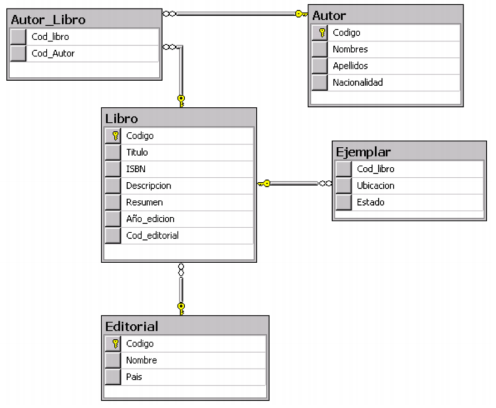
\includegraphics[width=13cm]{./images/1.png}
        \end{center}
        \begin{itemize}
            \item Creamos la \textbf{BD} usando el siguiente comando:
            \begin{center}
                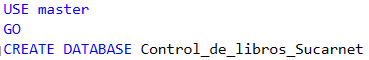
\includegraphics[width=13cm]{./images/1.1.png}
            \end{center}
            \newpage
            \item Creamos la tabla \textbf{Autor} usando el siguiente comando:
            \begin{center}
                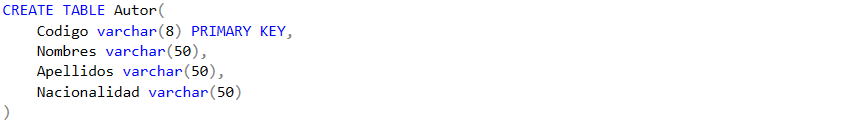
\includegraphics[width=13cm]{./images/1.2.png}
            \end{center}
            \item Creamos la tabla \textbf{Editorial} usando el siguiente comando:
            \begin{center}
                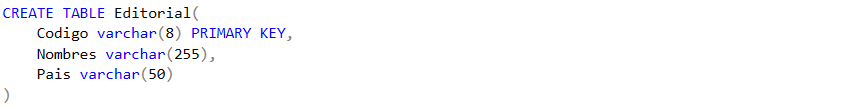
\includegraphics[width=13cm]{./images/1.3.png}
            \end{center}
            \item Creamos la tabla \textbf{Libro} usando el siguiente comando:
            \begin{center}
                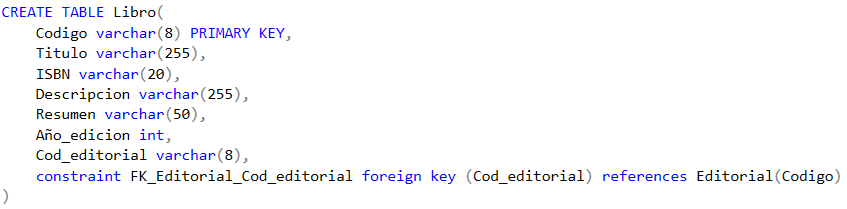
\includegraphics[width=13cm]{./images/1.4.png}
            \end{center}
            \item Creamos la tabla \textbf{Ejemplar} usando el siguiente comando:
            \begin{center}
                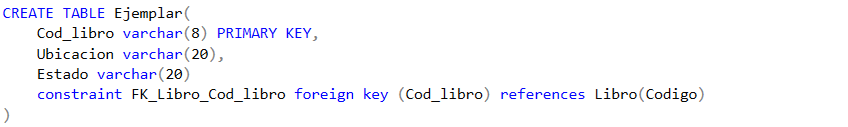
\includegraphics[width=13cm]{./images/1.5.png}
            \end{center}
            \item Creamos la tabla \textbf{Autor\_Libro} usando el siguiente comando:
            \begin{center}
                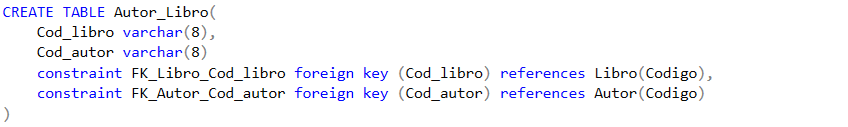
\includegraphics[width=13cm]{./images/1.6.png}
            \end{center}
        \end{itemize}
        \newpage
        \item Agregar los siguientes datos a cada tabla.
        \begin{itemize}
            \item Tabla Autor.s
            \begin{center}
                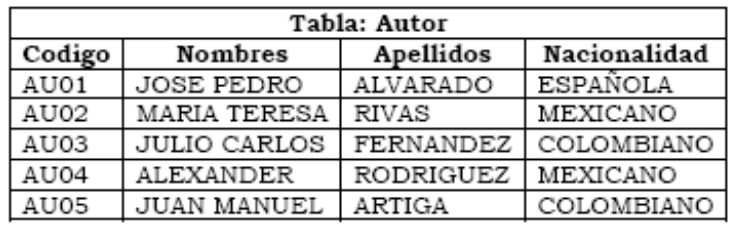
\includegraphics[width=13cm]{./images/2.png}
            \end{center}
            Para agregar los datos usar el siguiente codigo:
            \begin{center}
                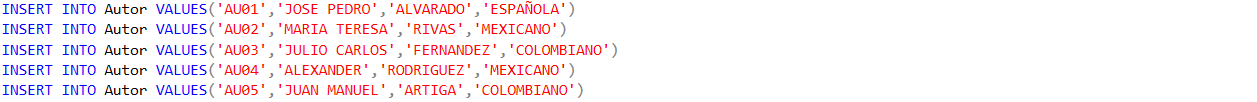
\includegraphics[width=13cm]{./images/2.1.png}
            \end{center}
            \item Tabla Editorial.
            \begin{center}
                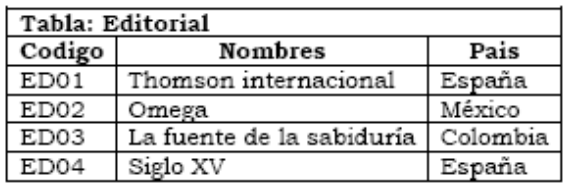
\includegraphics[width=13cm]{./images/3.png}
            \end{center}
            Para agregar los datos usar el siguiente codigo:
            \begin{center}
                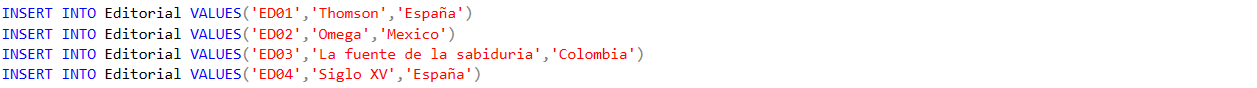
\includegraphics[width=13cm]{./images/3.1.png}
            \end{center}
            \newpage
            \item Tabla Libro.
            \begin{center}
                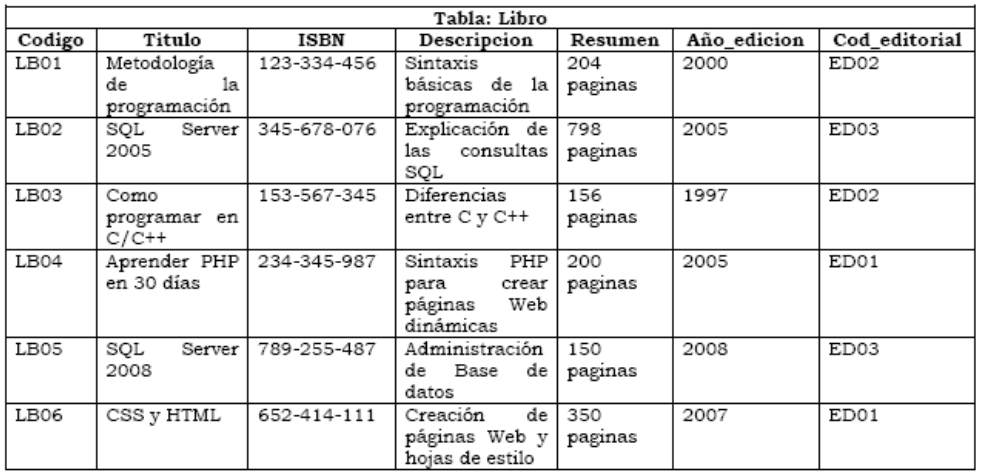
\includegraphics[width=13cm]{./images/4.png}
            \end{center}
            Para agregar los datos usar el siguiente codigo:
            \begin{center}
                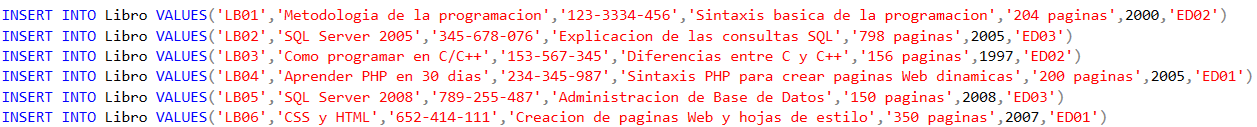
\includegraphics[width=13cm]{./images/4.1.png}
            \end{center}
            \newpage
            \item Tabla Ejemplar.
            \begin{center}
                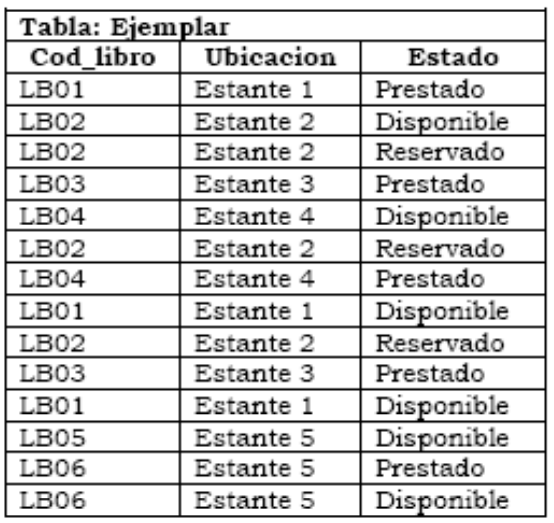
\includegraphics[width=13cm]{./images/5.png}
            \end{center}
            Para agregar los datos usar el siguiente codigo:
            \begin{center}
                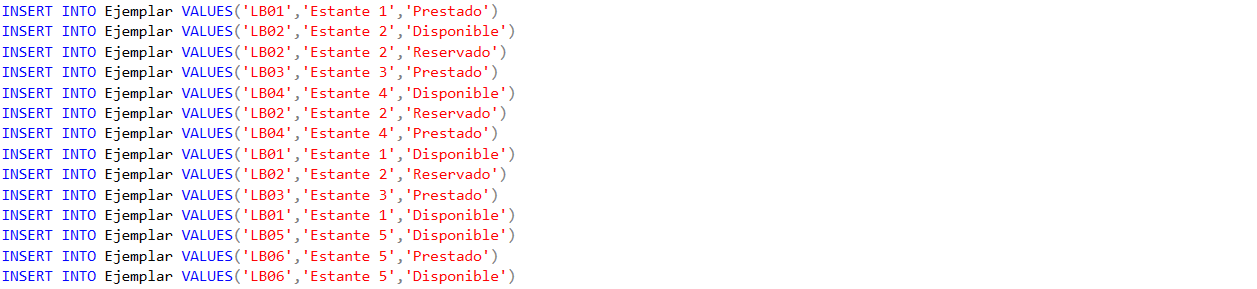
\includegraphics[width=13cm]{./images/5.1.png}
            \end{center}
            \newpage
            \item Tabla Autor\_Libro.
            \begin{center}
                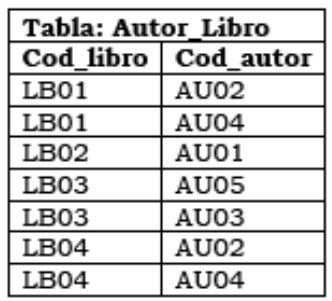
\includegraphics[width=13cm]{./images/6.png}
            \end{center}
            Para agregar los datos usar el siguiente codigo:
            \begin{center}
                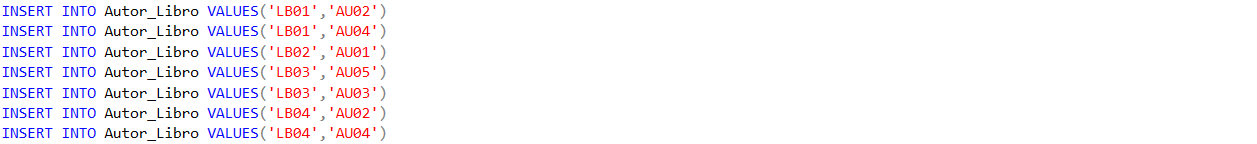
\includegraphics[width=13cm]{./images/6.1.png}
            \end{center}
        \end{itemize}
        \newpage
    \end{enumerate}
    
    \subsection{Parte II: Crear consultas SQL}
    Utilizando consultas a múltiples tablas resolver los siguientes problemas:
    \begin{enumerate}[\tab 1.]
        \item Se desea mostrar los datos de los autores junto con los títulos de libros que han escrito. Ordenarlos en forma descendente por el nombre del autor\\[0.1in]
        El codigo seria:
        \begin{center}
            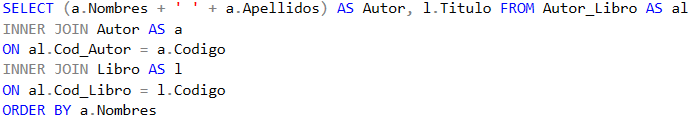
\includegraphics[width=13cm]{./images/7.1.png}
        \end{center}
        El resultado seria:
        \begin{center}
            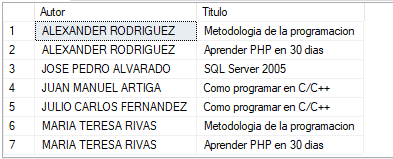
\includegraphics[width=13cm]{./images/7.2.png}
        \end{center}
        \item Se desea conocer todos los autores que tienen libros que han sido publicados por la editorial “Omega”.\\[0.1in]
        El codigo seria:
        \begin{center}
            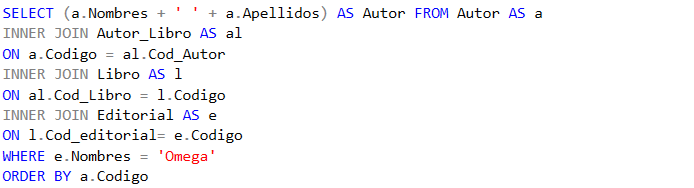
\includegraphics[width=13cm]{./images/8.1.png}
        \end{center}
        El resultado seria:
        \begin{center}
            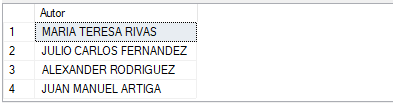
\includegraphics[width=13cm]{./images/8.2.png}
        \end{center}
        \item Mostrar cuántos ejemplares hay por cada libro. \textbf{Titulo, ejemplar}.\\[0.1in]
        El codigo seria:
        \begin{center}
            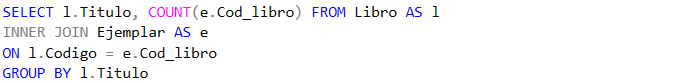
\includegraphics[width=13cm]{./images/9.1.png}
        \end{center}
        El resultado seria:
        \begin{center}
            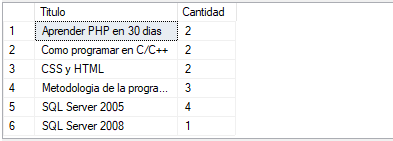
\includegraphics[width=13cm]{./images/9.2.png}
        \end{center}
        \item Mostrar los \textbf{títulos} de los libros donde el estado sea \textbf{“Prestado”}.\\[0.1in]
        El codigo seria:
        \begin{center}
            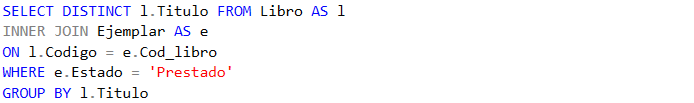
\includegraphics[width=13cm]{./images/10.1.png}
        \end{center}
        El resultado seria:
        \begin{center}
            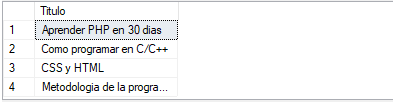
\includegraphics[width=13cm]{./images/10.2.png}
        \end{center}
        \item Se desea mostrar los libros que se han editados entre el \textbf{2000} y \textbf{2007}. Ordenarlos en forma ascendente.\\[0.1in]
        El codigo seria:
        \begin{center}
            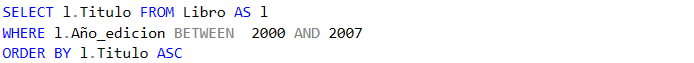
\includegraphics[width=13cm]{./images/11.1.png}
        \end{center}
        El resultado seria:
        \begin{center}
            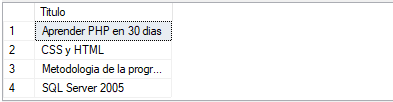
\includegraphics[width=13cm]{./images/11.2.png}
        \end{center}
        \item Mostrar cuántos libros que se han prestado y agruparlos por el estante\\[0.1in]
        El codigo seria:
        \begin{center}
            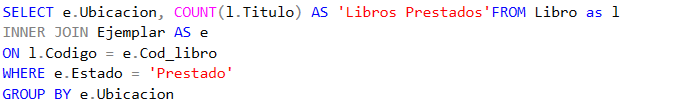
\includegraphics[width=13cm]{./images/12.1.png}
        \end{center}
        \newpage
        El resultado seria:
        \begin{center}
            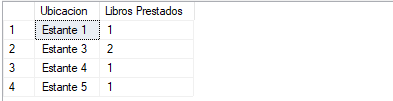
\includegraphics[width=13cm]{./images/12.2.png}
        \end{center}
    \end{enumerate}
    
    \subsection{Parte III: visualizador}
    Generar reportes operacionales de la parte II utilizando un visualizador Power BI, Tableau o Qlik Sense.
    \begin{enumerate}[\tab 1.]
        \item Se desea mostrar los datos de los autores junto con los títulos de libros que han escrito. Ordenarlos en forma descendente por el nombre del autor
        \begin{center}
            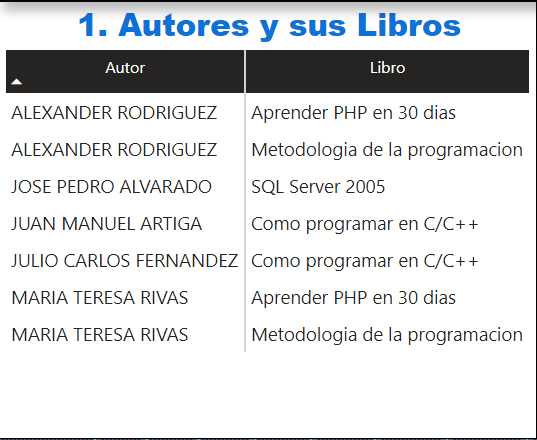
\includegraphics[width=13cm]{./images/13.png}
        \end{center}
        \newpage
        \item Se desea conocer todos los autores que tienen libros que han sido publicados por la editorial “Omega”.
        \begin{center}
            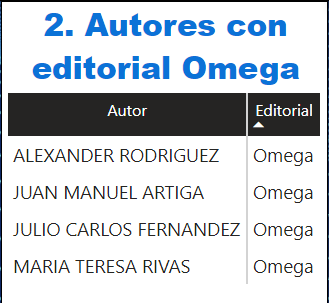
\includegraphics[width=13cm]{./images/14.png}
        \end{center}
        \newpage
        \item Mostrar cuántos ejemplares hay por cada libro. \textbf{Titulo, ejemplar}.
        \begin{center}
            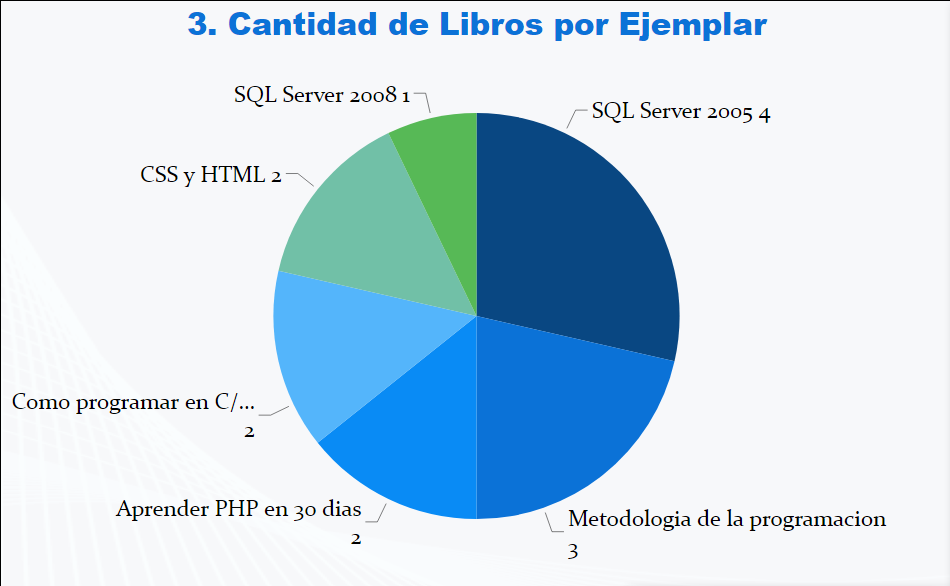
\includegraphics[width=13cm]{./images/15.png}
        \end{center}
        \newpage
        \item Mostrar los \textbf{títulos} de los libros donde el estado sea \textbf{“Prestado”}.
        \begin{center}
            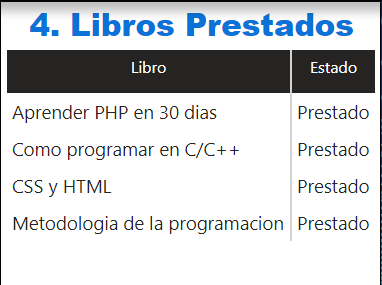
\includegraphics[width=13cm]{./images/16.png}
        \end{center}
        \newpage
        \item Se desea mostrar los libros que se han editados entre el \textbf{2000} y \textbf{2007}. Ordenarlos en forma ascendente.
        \begin{center}
            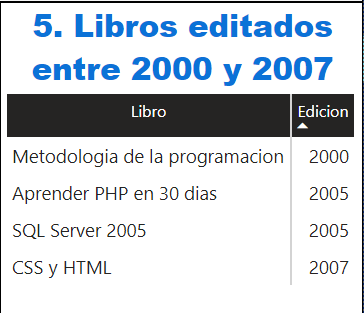
\includegraphics[width=13cm]{./images/17.png}
        \end{center}
        \item Mostrar cuántos libros que se han prestado y agruparlos por el estante
        \begin{center}
            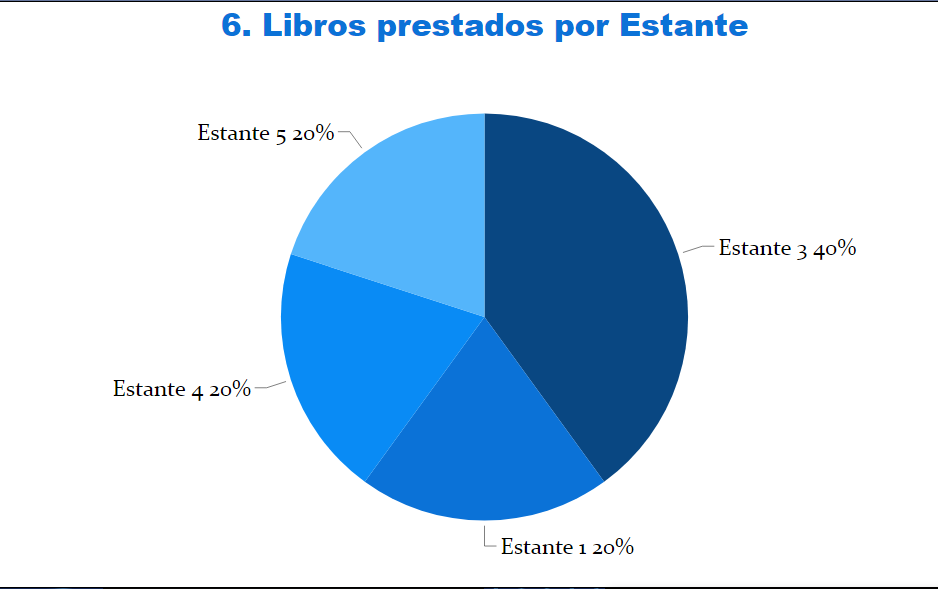
\includegraphics[width=13cm]{./images/18.png}
        \end{center}
    \end{enumerate}
    \newpage
    Finalmente nuestro dashboard se veria de la siguiente manera con todos los reportes solicitados.
    \begin{center}
        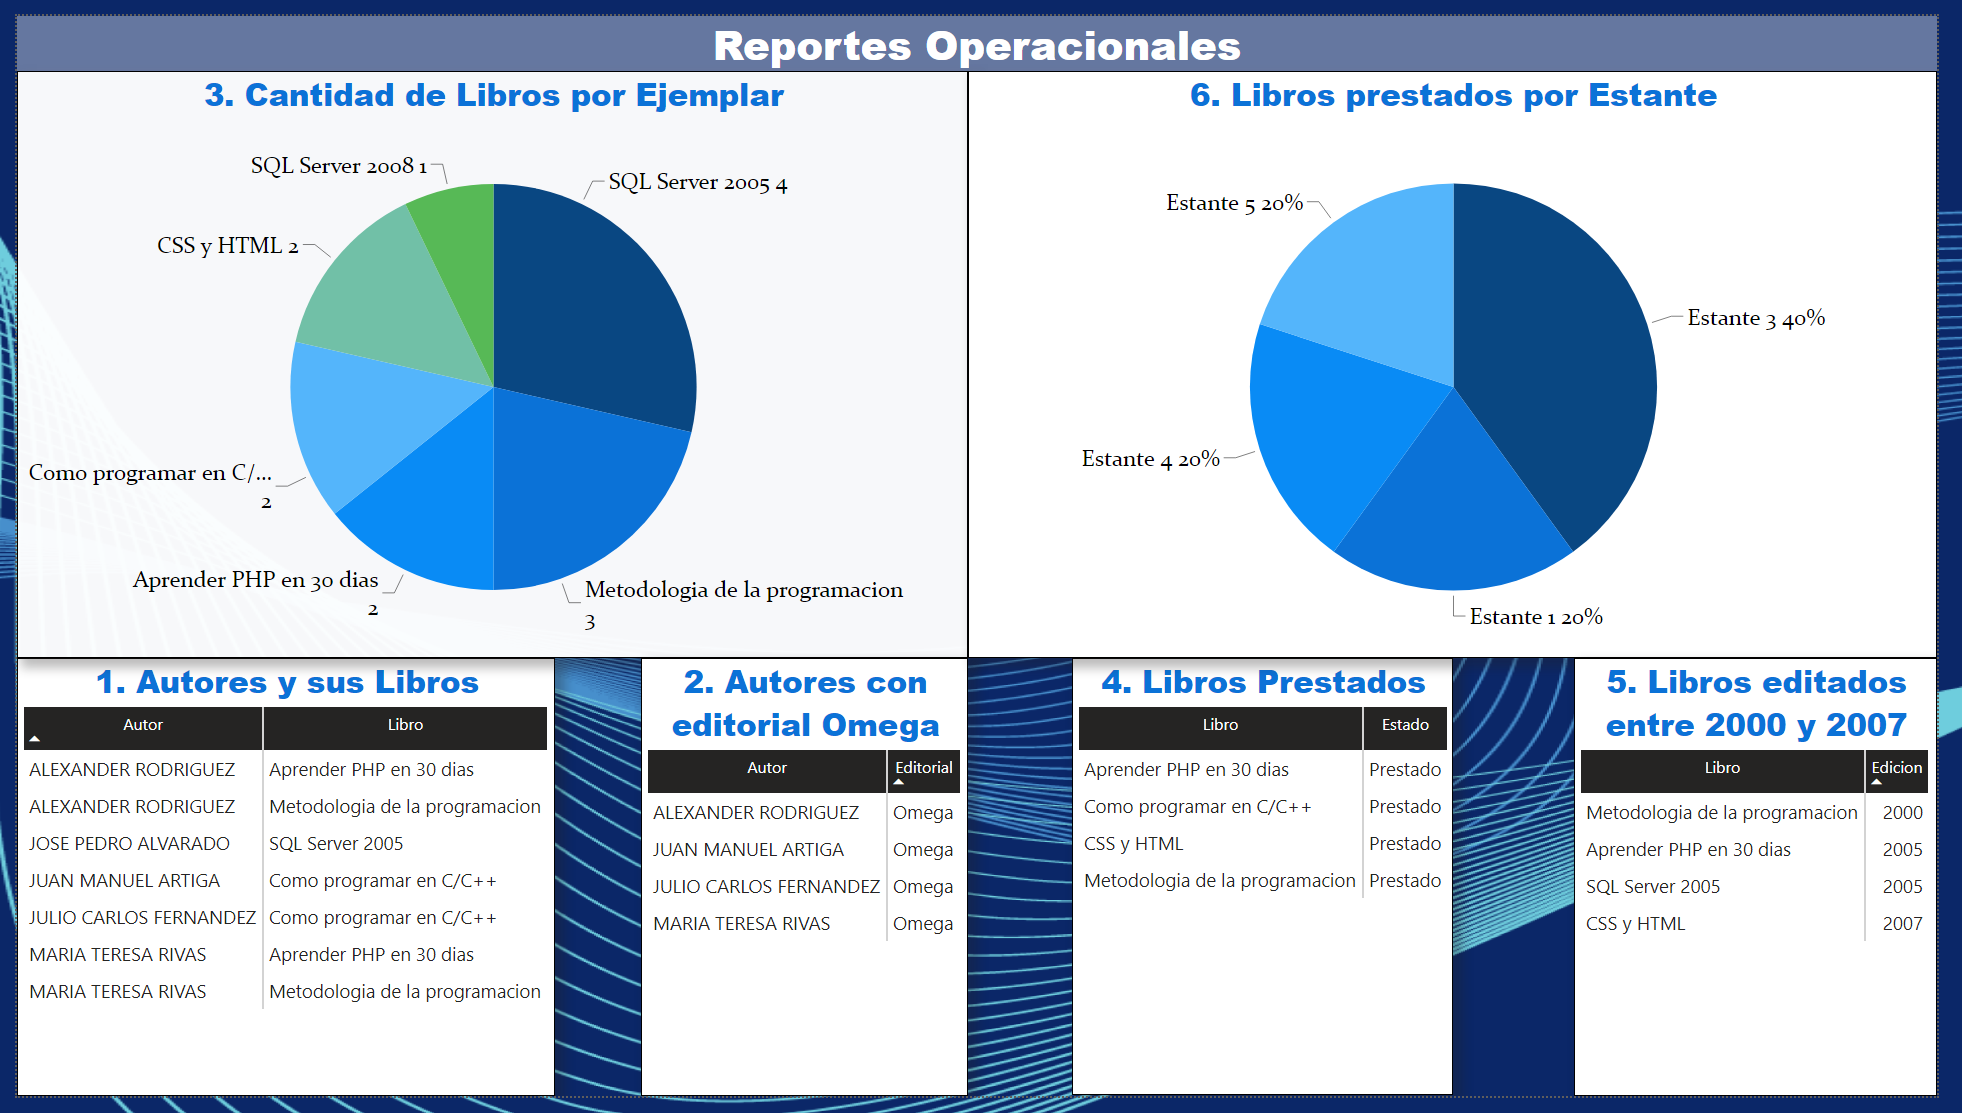
\includegraphics[width=18cm]{./images/19.png}
    \end{center}

	
\end{document}